\documentclass{article}
\usepackage[utf8]{inputenc}
\usepackage{parskip}
\usepackage{lmodern}
\usepackage[T1]{fontenc}
\usepackage[english]{babel}
\usepackage{amsmath}
\usepackage{amsthm}
\usepackage{amssymb}
\usepackage{graphicx}

\begin{document}

{\large
Elli Kiiski
\par
An exercise from the course History of Mathematics\\University of Helsinki
}
\vspace{0.5cm}

\section*{Area of lune}

Lune of Hippocratus is a shape bounded by arcs of two circles, as shown in the picture here.
\begin{figure}[!htb]
    \centering
    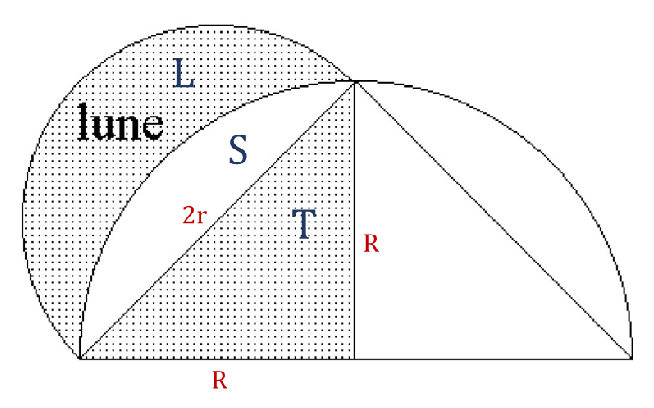
\includegraphics[width =55mm]{lune.eps}
\end{figure}

Let $R$ be the radius of the bigger circle and $r$ the radius of the smaller. Also, let $T$, $S$ and $L$ equal the areas of the triangle, segment and lune respectively (see the picture).

By simple geometry, we have
\begin{equation*}
\label{radius}
    2r=\sqrt{2}R \Leftrightarrow r=\frac{\sqrt{2}}{2}R
\end{equation*}
and
\begin{equation*}
\label{segment}
    S = \frac{1}{4}\pi R^2 - T.
\end{equation*}
Finally, we get
\begin{equation*}
    L = \frac{1}{2}\pi r^2 - S = \frac{1}{2}\pi (\frac{\sqrt{2}}{2}R)^2 - S = \frac{1}{4}\pi R^2 - (\frac{1}{4}\pi R^2 - T) = T.
\end{equation*}
Hence that area of the lune ($L$) equals the area of the triangle ($T$).

\end{document}
